%!TEX root = sdm-2018.tex
\section{Experiments}
\label{sec:experiments}

% \textbf{Graphs}

% \begin{itemize}
% 	\item ASS1 \\
% 	Nodes: 3015\\
% 	Edges: 5539

% 	\item GEO \\
% 	Nodes: 1000 \\
% 	Unit square with random nodes. Nodes within 0.01 distance are connected.

% 	\item GRID \\
% 	Nodes: 1000 \\
% 	All nodes except ones on border have out-degree and in-degree 4

% 	\item BA \\
% 	Nodes: 1000 \\
% 	preferential attachment parameter: 10, 5, 3. Results are for 10, but they don't change qualitatively for any other parameter.
% \end{itemize}
% \textbf{Item distributions}
% \begin{itemize}
% 	\item Uniform \\
% 	Items per node is total items / total nodes

% 	\item Direct \\
% 	Items directly proportional to out-degreee

% 	\item Inverse \\
% 	Items inversely proportional to out-degree. (directly proportional to number of nodes that are not the neighbors of given node.) \\
% 	Very similar to Uniform in sparse graphs.

% 	\item Ego \\
% 	Randomly chosen node. 70\% items distributed in a 2-radius sphere around randomly chosen node. 30\% outside. \\
% 	All results are averaged over 10 runs.

% \end{itemize}
In this section, we describe the results of our experimental evaluation using
real and synthetic data. The results demonstrate that our methods
perform better than other baseline methods with respect to our objective function. 
Moreover, using the bike-sharing network of Boston,
we provide anecdotal evidence that our methods pick meaningful nodes
to monitor.


\subsection{Experimental setup}

Let us first describe the experimental setup, i.e., the 
datasets and baseline algorithms used for evaluation.

\spara{Graph datasets:} We use the following graphs to 
define {\markovchain}s for our experiments.

\emph{\autonomoussystems} is a graph that contains information about 
traffic  between \textit{Autonomous Systems} of the Internet. 
%(An Autonomous System (AS)
%can be thought of as a set of IP addresses, 
%typically characterized by their common prefix 
%and belonging to a single internet provider or large organization). 
The dataset was retrieved through the Stanford Large Network Dataset 
Collection (SNAP)~\cite{snapnets}.
We experimented with three snapshots of the %Autonomous Systems
communication graphs between years 1997 and 2000. 
Here we demonstrate results for one of the snapshots (1999-2000), 
as we did not find significant difference among them.

The {\autonomoussystems} graph contains one node for each 
AS. Moreover, for every pair of nodes between which there is traffic according
to the dataset, we place two directed edges between the nodes, one in
each direction. To create an instance of the transition matrix,
we assign equal probabilities to the outgoing edges of each node.

\emph{{\grid} graphs:} The {\grid} graphs are 
planar, bi-directed grid graphs, 
where each node has in- and out-degree $4$ 
(with the exception of border nodes). 


\emph{{\geo} graphs:} The {\geo} graphs are 
bi-directed geographic graphs. They are generated as follows:
each node is placed randomly within a unit square 
on the two-dimensional euclidean plane.
Subsequently, pairs of nodes are connected with directed edges in both
directions if their euclidean distance is below a pre-defined threshold
$ds = 0.01$. 


\emph{{\ba} graphs}: The {\ba} graphs are  generated according to the
Barabasi-Albert model. According to the model,
nodes are added to the graph incrementally one after the other, 
each of them with outgoing edges to $m$ existing nodes selected
via preferential attachment. Here we show results for $m=3$, but the results
were similar for values $m=5,10$. 

Similar to the methodology of Gionis {\etal}~\cite{gionis2015bump}, 
the {\grid}, {\geo} and {\ba} graphs provide us 
with different varieties of synthetic graphs to explore the performance 
our methods.

\spara{Item distributions:}
For each aforementioned graph, we generate an initial distribution
of items \initial\ according to one of the following four schemes.

%\begin{itemize}
\squishlist
\item \ego. Items are assigned in two steps. Firstly, one node
	is selected uniformly at random among all nodes. Secondly,
	$70\%$ of items are assigned randomly on the neighbors of the selected node
	(including the selected node itself). Finally, the remaining items
	are distributed randomly to the nodes outside the neighborhood of the 
	selected node.
\item \uniform. Each node is assigned the same number of items.
\item \direct. The number of items on each node is directly proportional to its
	out-degree. Note that items are distributed in a deterministic manner.
\item \inverse. The number of items on each node is assigned deterministically to
	be inversely proportional to its out-degree.
\squishend
%\end{itemize}

Now each graph described above is combined with 
each item-distribution scheme. 
As a result, we obtain datasets of the form {\tt G-X}, where 
{\tt G} is any of {\autonomoussystems}, {\grid},  {\geo} and {\ba} 
and {\tt X} is any of the {\ego}, {\uniform}, {\direct} and {\inverse}.
For simplicity, for the datasets that are generated randomly, 
we perform experiments over a single fixed instantiation.


\spara{The {\hubway} dataset:} Hubway
is a bike-sharing system in the Boston metro area, with a fleet of 
over 1000 bikes and over 100 hubway stations where users can pick up or 
drop off bikes at.
Every time a user picks up a bike from a Hubway station, 
the system records basic
information about the trip, such as the pick-up and drop-off
station, and the corresponding pick-up and drop-off times. 
Moreover, the data contain the number of available bikes
at each Hubway station every minute. 
The dataset was made publicly available by Hubway for the purposes of
its Data Visualization 
Challenge\footnote{http://hubwaydatachallenge.org/}.

Using the dataset, we create instances of the problems we consider as follows.
Firstly, we create a complete graph by representing each station with one
node in the graph, and considering all possible edges between them.
Subsequently, we consider a time interval $(t_s, t_e)$ and the bikes that
are located at each station (node). 
Representing bikes as items in our setting, we assign a transition 
probability $\transition(u,v)$ between nodes $u$ and $v$ by considering the 
total number $n_u$ of bikes at station $u$ at start time $t_s$ and, among these bikes,
the number $n_{uv}$ of them that were located at station $v$ at end time $t_e$.
We then set $\transition(u,v) = n_{uv}/n_u$ and ignore edges with zero
transition probability.

We experimented with a large number of such instances for different intervals
$(t_s, t_e)$, with a moderate length of $2$ hours, to capture real-life
transitions from one node to another. For the experiments presented in the 
paper, we use a fixed instance for the interval between 10am and 12pm on
April 1st, 2012. In this interval, we consider 61 stations with at least one trip
starting or ending at each. We refer to the dataset so constructed as the {\hubway}
dataset.

\spara{Baseline algorithms:}
In order to assess the performance of our proposed algorithms for the
{\nodeproblem} and {\edgeproblem} problem variants,
we compare it to that of well-known baseline algorithms from
the literature. Since we are the first to tackle the problem of
\mcproblem, the baseline algorithms we compare with do not target our objective
function directly. Nevertheless, the comparison helps us highlight the settings
in which our algorithms are essential to achieve good performance
for \mcproblem.

Below, we describe the respective baselines for the two variants of the problem.


\emph{Baselines for {\nodeproblem}:} For a budget $k$, the following baselines
return a set of $k$ nodes with highest value for the respective measure:
%\begin{itemize}
\squishlist
	\item {\indegree}: number of incoming edges;
	\item {\inprobability}: total probability of incoming edges;
	\item {\nodebetweenness}: as defined in~\cite{brandes01faster,erdos15divide,riondato16fast};
	\item {\closeness}: as defined in~\cite{sabidussi1966centrality};
	\item {\nodenumitems}: number of items before transition;
	%\item {\pagerank}: PageRank of the node~\cite{pagerank1999}.
%\end{itemize}
\squishend
	% The {\betweenness} and {\closeness}
	% heuristics choose top-$k$ nodes sorted using their betweenness and 
	% closeness centrality measures
	% respectively. Finally, the {\numitems} baseline chooses $k$ nodes with 
	% highest items.

\emph{Baselines for {\edgeproblem}:}. For a budget $k$, the following baselines
return a set of $k$ edges with highest value for the respective measure:
%\begin{itemize}
\squishlist
	\item {\edgebetweenness}: as defined in~\cite{brandes01faster,erdos15divide,riondato16fast};
	\item {\edgenumitems}: expected number of items to transition over the edge;
	\item {\probability}: transition probability of the edge.
\squishend
%\end{itemize}

% \spara{Note:} The same name is used for some baselines across problem variants
% (\betweenness, \numitems).
In what follows, context determines which baseline and variant we refer to.



\iffalse
=====
the datasets and the experiments used for 
evaluating the proposed algorithms. 
The experiments compare our methods for both {\nodeproblem} and 
{\edgeproblem} problems with baseline methods from related work. 
We use five datasets to create instances of graphs and transition
probabilities,
two real ones (namely {\hubway} and {\autonomoussystems}), 
and three synthetic ones (namely {\grid}, {\geo}, and {\ba}). 
Subsequently, to explore the behavior of algorithms under different 
distributions of items, we consider four ways to synthetically
distribute items among the nodes.
They are described below.





% \todo[HC]{Check time information above.}
% \todo[HC]{Check and include information on number of stations in our dataset.}

% In our setting, we look at the each Hubway station in Boston as a node of the graph and the available bikes
% at that station as the number of items on that node. There exists a directed edge from node $u$ to node $v$ of the graph if
% there has been at least one bike ride starting from node $u$ and ending at node $v$ in the given time frame. 
% We use the number of rides between each pair of stations to build a transition matrix. 
% \todo{How? We need to describe the discretization into timesteps.} 
% Since it is possible to take a bike ride between every pair of the stations, the graph $G$ formed using the bike rides could possibly be a complete graph. However, due to external factors such as terrain, traffic and road networks, the resulting transition matrix is sparse.


% In our setting we look at each Autonomous System as a node of the graph. Every undirected edge between nodes $u$ and $v$ is replaced
% by two directed edges in either direction. For the resulting network, we assign equal probabilities to every outgoing edge from every node, to generate a transition matrix. As there is no readily available information about the number of packets flowing from one Autonomous System to another, we combine the real graph between the Autonomous Systems with synthetically generated distribution of items across the nodes.
% Specifically, for a given total number of items, we consider the following three distributions:
% % number of routers comprising each of the Autonomous Systems to use as items in our setting, we take as an user input the total number of items, and evaluate our algorithms on three different kinds of item distributions over nodes.
% \begin{itemize}
% 	\item {\uniform} Number of items on each node is equal. 
% 	\item {\direct} Number of items on each node is directly proportional to its out-degree. 
% 	\item {\inverse} Number of items on each node is inversely proportional to its out-degree. 
% \end{itemize}




% The {\betweenness} baseline choses top-$k$ edges with based on their
% 	betweenness centrality while the {\numitems} baseline chooses $k$ edges with highest
% 	expected number of items to transition along them. The {\probability} baseline simply
% 	chooses $k$ highest probability edges.
% \end{itemize}

% \begin{itemize}
% 	\item Uniform \\
% 	Items per node is total items / total nodes

% 	\item Direct \\
% 	Items directly proportional to out-degree

% 	\item Inverse \\
% 	Items inversely proportional to out-degree. (directly proportional to number of nodes that are not the neighbors of given node.) \\
% 	Very similar to Uniform in sparse graphs.

% 	\item Ego \\
% 	Randomly chosen node. 70\% items distributed in a 2-radius sphere around randomly chosen node. 30\% outside. \\
% 	All results are averaged over 10 runs.

% \end{itemize}

% Node plots

\fi

% Hubway Plots




%\begin{figure}
%	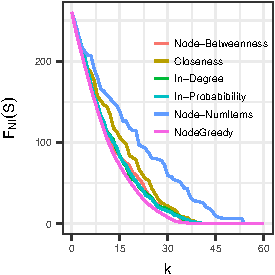
\includegraphics{figures/hubway_nodes.pdf}
%	\caption{Hubway node objective evolution.}
%	\label{fig:hubway_nodes}
%\end{figure}
%
%\begin{figure}
%	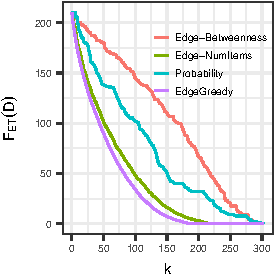
\includegraphics{figures/hubway_edges.pdf}
%	\caption{Hubway edge objective evolution.}
%	\label{fig:hubway_edges}
%\end{figure}


\begin{table*}[htbp]\small
\centering
\begin{tabular}{@{}llcccc@{}}
\toprule
\multirow{2}{*}{\begin{tabular}[l]{@{}l@{}}Graph\end{tabular}}                                                                         & \multirow{2}{*}{\begin{tabular}[l]{@{}l@{}}Item\\Distribution\ \ \ \ \ \ \end{tabular}} & \multirow{2}{*}{\begin{tabular}[l]{@{}l@{}}$r({\nodegreedy})$\end{tabular}} & \multirow{2}{*}{\begin{tabular}[l]{@{}l@{}}$r({\tt Node-Baseline}^\ast)$\end{tabular}} & \multirow{2}{*}{\begin{tabular}[l]{@{}l@{}}$r({\edgegreedy})$\end{tabular}} & \multirow{2}{*}{\begin{tabular}[l]{@{}l@{}}$r({\tt Edge-Baseline}^\ast)$\end{tabular}}\\ \\ \toprule
\multirow{4}{*}{\begin{tabular}[l]{@{}l@{}}{\autonomoussystems}\end{tabular}}  & {\ego}               & 0.06                                  & 0.24                                   & 0.14                                  & 0.15                                   \\
                                                                               & {\direct}            & 0.66                                  & 0.67                                   & 0.99                                  & 0.99                                   \\
                                                                               & {\uniform}           & 0.38                                  & 0.40                                   & 0.97                                  & 0.99                                   \\
                                                                               & {\inverse}           & 0.38                                  & 0.40                                   & 0.97                                  & 0.99                                   \\ \cmidrule(l){2-6}
\multirow{4}{*}{\begin{tabular}[l]{@{}l@{}}{\geo}\end{tabular}} 			   & {\ego}               & 0.00                                  & 0.06                                   & 0.01                                  & 0.02                                   \\
                                                                               & {\direct}            & 0.00                                  & 0.06                                   & 0.20                                  & 0.65                                   \\
                                                                               & {\uniform}           & 0.00                                  & 0.06                                   & 0.15                                  & 0.65                                   \\
                                                                               & {\inverse}           & 0.00                                  & 0.07                                   & 0.15                                  & 0.65                                   \\ \cmidrule(l){2-6}
\multirow{4}{*}{\begin{tabular}[l]{@{}l@{}}{\grid}\end{tabular}} 	           & {\ego}               & 0.27                                  & 0.27                                   & 0.29                                  & 0.29                                   \\
                                                                               & {\direct}            & 0.92                                  & 0.92                                   & 0.98                                  & 0.98                                   \\
                                                                               & {\uniform}           & 0.92                                  & 0.92                                   & 0.98                                  & 0.98                                   \\
                                                                               & {\inverse}           & 0.92                                  & 0.92                                   & 0.98                                  & 0.98                                   \\ \cmidrule(l){2-6}
\multirow{4}{*}{\begin{tabular}[l]{@{}l@{}}{\ba}\end{tabular}} 	               & {\ego}               & 0.18                                  & 0.56                                   & 0.26                                  & 0.26                                   \\
                                                                               & {\direct}            & 0.71                                  & 0.71                                   & 0.99                                  & 0.99                                   \\
                                                                               & {\uniform}           & 0.63                                  & 0.63                                   & 0.98                                  & 0.98                                   \\
                                                                               & {\inverse}           & 0.63                                  & 0.63                                   & 0.98                                  & 0.98                                   \\ \bottomrule                                                                             
\end{tabular}
\caption{Comparison of greedy algorithms with the best-performing baseline (${\tt Node-Baseline}^\ast$ and ${\tt Edge-Baseline}^\ast$) for $k=50$. 
For a given pair of graph and item-distribution scheme, $r(A)$ expresses the 
ratio of the expected uncertainty that algorithm $A$ achieves with $k=50$
monitoring operations over the initial uncertainty $\uncertainty_0$ 
(for $k=0$). Note that the best-performing baseline is different for different rows of the table.
}
\label{tab:objective-evolution-table}
\end{table*}

%\begin{table}[htbp]
%\centering
%\begin{tabular}{@{}ll@{}}
%\toprule
%ID & Landmark                           \\ \toprule
%33 & Kenmore Sq.                        \\
%36 & Copley Sq./Boston Public Library \\
%41 & Packard's Corner                   \\
%42 & Boston Public Garden               \\
%52 & Newbury St.                        \\ \bottomrule
%\end{tabular}
%\caption{Hubway stations in Boston city minimizing uncertainty (k=5).}
%\label{tab:hubway-table}
%\end{table}

% For both {\nodeproblem} and {\edgeproblem} problems, the number of items allocated to each node during initialization are chosen using three criteria,
% \begin{itemize} 
% 	\item Uniformly distributed over nodes.
% 	\item Directly proportional to the out-degree of the node.
% 	\item Inversely proportional to the out-degree of the node.
% \end{itemize}
% For each of the above three item initializations, we compare the following baseline approaches of choosing 'k' nodes,
% \begin{itemize}
% 	\item {\nodeproblem} baselines
% 	\begin{itemize}
% 		\item $k$ randomly chosen nodes.
% 		\item Top-$k$ nodes of highest incoming probabilities.
% 		\item Top-$k$ nodes of highest in-degree centrality scores.
% 		\item Top-$k$ nodes of highest degree-centrality scores.
% 		\item Top-$k$ nodes chosen using {\nodegreedy} algorithm.
% 	\end{itemize}
% 	\item {\edgeproblem} baselines
% 	\begin{itemize}
% 		\item $k$ randomly chosen edges.
% 		\item Top-$k$ edges of highest probabilities.
% 		\item Top-$k$ edges chosen using {\edgegreedy} algorithm.
% 	\end{itemize}
% \end{itemize}
% For each of the configurations described above, we make following two plots,
% \begin{itemize}
% 	\item Evolution of objective function value for $k=0$ over time. (At some time, the items distribution over nodes approaches the stationary distribution. The objective function value for $k=0$ remains constant thereafter.)

% 	\item Evolution of objective function value over different values of $k$. (As the $k$ increases, the uncertainty should decrease ultimately to zero.)

% \end{itemize}



\begin{figure}
\begin{subfigure}[b]{0.23\textwidth}
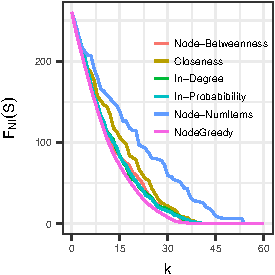
\includegraphics[width=\textwidth]{figures/hubway_nodes.pdf}
\caption{{\nodeproblem}}
\label{fig:hubway_nodes}
\end{subfigure}
\begin{subfigure}[b]{0.23\textwidth}
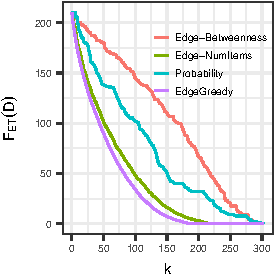
\includegraphics[width=\textwidth]{figures/hubway_edges.pdf}
\caption{{\edgeproblem}}
\label{fig:hubway_edges}
\end{subfigure}
\caption{{\hubway} data; $y$-axis: expected uncertainty, $x$-axis: number of monitored nodes or edges.}
\end{figure}



\subsection{Experimental results}
In this section, we report the   
performance of algorithms for the {\mcproblem} problem -
first on the graph datasets, combined with item distribution schemes;
then on the \hubway\ dataset.
As objective we always use the expected uncertainty
achieved for a given budget $k$ of nodes or edges -- the smaller its value,
the better the performance of the algorithm.
Note that we do not report separately the performance of \edgeDP, as it achieves
same performance as \edgegreedy, but is not as efficient.


We provide the results for the graph datasets in Table \ref{tab:objective-evolution-table}. 
In all these experiments we use $k=50$.
Moreover, $r(A)$ is the ratio of the achieved objective value (for $k=50$) over
the initial value $\uncertainty_0$ of the measure 
(for no monitoring operations, i.e., $k=0$).
The table shows four quantities for every graph-item distribution pair
: $r(A)$ for $A=\{${\nodegreedy}, {\tt Node-Baseline}$^\ast$, {\edgegreedy}, {\tt Edge-Baseline}$^\ast$ $\}$.
Note that {\tt Node-Baseline}$^\ast$ (resp.\ {\tt Edge-Baseline}$^\ast$) refers to the baseline 
algorithm with the best performance.
For every algorithm $A$, $r(A)\in[0,1]$ and the smaller the value of $r(A)$ the better the performance of the algorithm.
 
From the table, we observe that for 
the {\autonomoussystems} dataset,  {\nodegreedy}  significantly outperforms the best
baseline for the {\ego} item distribution, while performing marginally better for other item distributions.
The value of  $r({\edgegreedy})$ is only slightly less than
the best baselines across all the configurations. However, we observe that there is no baseline
which performs uniformly the best across different item distributions. For example,  {\edgebetweenness}
is the best baseline for {\direct} item distribution, the {\edgenumitems} for {\ego}, while they both
perform worse than even randomly chosen edges for {\uniform} and {\inverse} item distributions.
Notably, for the {\geo} graphs, the greedy algorithms significantly outperform the baselines


For the {\grid} graphs, the baselines perform exactly
the same as our algorithms. This can be explained by the nature of the 
{\grid} graph, where all the nodes except the ones on the boundary are similar to each other,
thereby rendering the {\direct}, {\uniform} and {\inverse} item distributions very similar 
to each other. For the {\ego} distribution, the greedy algorithms perform marginally better
than the baselines.
%, depending on the number of nodes within the fixed radius around the randomly chosen node, 
%and the percentage of items distributed among these nodes. 
Again,
there is no baseline which performs uniformly the best.
Similar is our explanation for the results on {\ba} graphs as in these graphs most of the nodes have
almost the same (small) degrees too.

A more thorough investigation of the performance of the algorithms for different
values of $k$ and for all datasets we consider is shown in 
Supplementary Material, Section~\ref{sec:additional_results}.





\spara{Experiments with {\hubway} data:}
In our last experiment, 
we explore the performance of our algorithms on the {\hubway} dataset. From Figure \ref{fig:hubway_nodes}
and Figure \ref{fig:hubway_edges} we observe that the {\nodegreedy} and {\edgegreedy} algorithms
are consistently the best at reducing expected uncertainty, although the baselines are competitive on the
relatively smaller graph. In Figure \ref{fig:hubway_stations}, we plot the Hubway stations across Boston
chosen by the {\nodegreedy} algorithm with $k=5$. The nodes chosen by the algorithm are supported by
the anecdotal evidence of being exactly some of the of the most popular landmarks around the city.
From a managerial perspective, tracking the number of trips starting or ending at these Hubway stations
can help the operators better reduce the expected uncertainty around the expected number of bikes
available at its different stations and anticipate future bike ``re-balancing"\footnote{https://www.citylab.com/transportation/2014/08/balancing-bike-share-stations-has-become-a-serious-scientific-endeavor/379188/} operations.

\spara{Running times:} For all our experiments we use a single process 
implementation of our algorithms on a 24-core 2.9GHz Intel Xeon E5 processor 
with 512GB memory. For the  largest graph in our experiments,  
the parallelized version of the {\nodegreedy}\ takes about $5-10$ 
seconds per selected node, while the parallelized version of {\edgegreedy}\ 
takes about $1$ minute per selected edge.

\begin{figure}
	\centering
	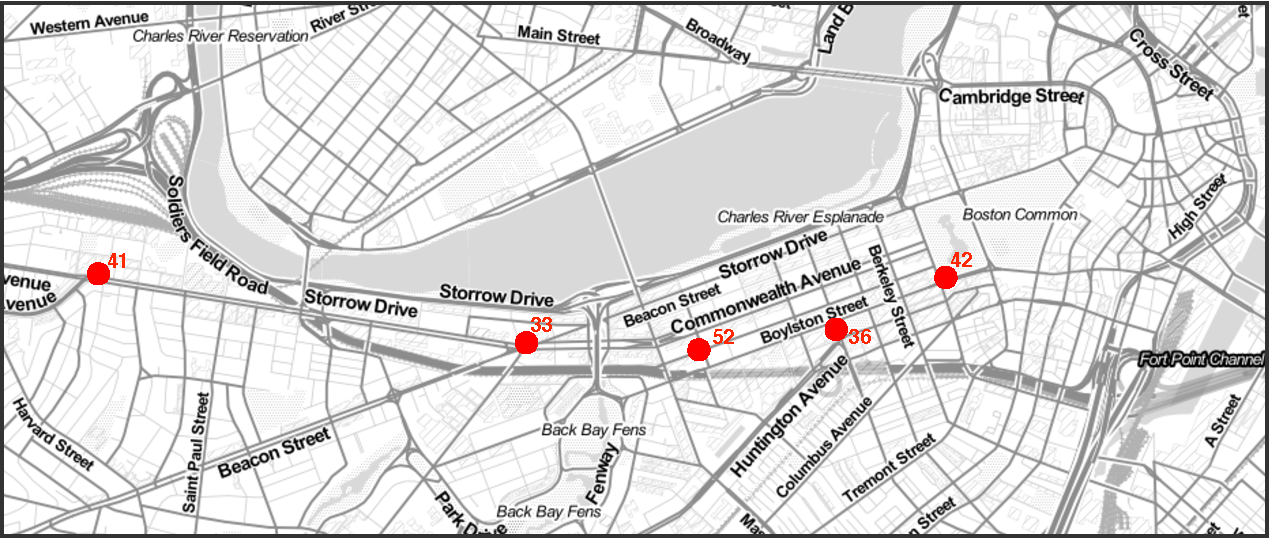
\includegraphics[width=8cm, height=4cm]{figures/hubway_stations_5.pdf}
	\caption{{\hubway} data. IDs of stations picked as a solution to {\nodeproblem}
	for $k=5$;
	33: Kenmore Sq., 36: Copley Sq./Boston Public Library, 41: Packard's Corner, 
	42: Boston Public Garden, 52: Newbury St.                        }
	\label{fig:hubway_stations}
\end{figure}


\spara{Discussion:} Our experiments show that  {\nodegreedy} and  {\edgegreedy} 
consistently perform better than or on par with other popular baseline methods. Also, for 
graphs with relatively large number of nodes, the solutions to the {\nodeproblem} problem 
are more effective at reducing
the expected uncertainty than the solutions to the {\edgeproblem} problem for the same number of
node (resp.\ edge) monitors.
This is
especially important considering our analysis from Section \ref{sec:nodes} and \ref{sec:edges} which show
that the {\nodegreedy} algorithm has a better time complexity compared to the {\edgegreedy} for dense graphs.

